\documentclass[1p]{elsarticle_modified}
%\bibliographystyle{elsarticle-num}

%\usepackage[colorlinks]{hyperref}
%\usepackage{abbrmath_seonhwa} %\Abb, \Ascr, \Acal ,\Abf, \Afrak
\usepackage{amsfonts}
\usepackage{amssymb}
\usepackage{amsmath}
\usepackage{amsthm}
\usepackage{scalefnt}
\usepackage{amsbsy}
\usepackage{kotex}
\usepackage{caption}
\usepackage{subfig}
\usepackage{color}
\usepackage{graphicx}
\usepackage{xcolor} %% white, black, red, green, blue, cyan, magenta, yellow
\usepackage{float}
\usepackage{setspace}
\usepackage{hyperref}

\usepackage{tikz}
\usetikzlibrary{arrows}

\usepackage{multirow}
\usepackage{array} % fixed length table
\usepackage{hhline}

%%%%%%%%%%%%%%%%%%%%%
\makeatletter
\renewcommand*\env@matrix[1][\arraystretch]{%
	\edef\arraystretch{#1}%
	\hskip -\arraycolsep
	\let\@ifnextchar\new@ifnextchar
	\array{*\c@MaxMatrixCols c}}
\makeatother %https://tex.stackexchange.com/questions/14071/how-can-i-increase-the-line-spacing-in-a-matrix
%%%%%%%%%%%%%%%

\usepackage[normalem]{ulem}

\newcommand{\msout}[1]{\ifmmode\text{\sout{\ensuremath{#1}}}\else\sout{#1}\fi}
%SOURCE: \msout is \stkout macro in https://tex.stackexchange.com/questions/20609/strikeout-in-math-mode

\newcommand{\cancel}[1]{
	\ifmmode
	{\color{red}\msout{#1}}
	\else
	{\color{red}\sout{#1}}
	\fi
}

\newcommand{\add}[1]{
	{\color{blue}\uwave{#1}}
}

\newcommand{\replace}[2]{
	\ifmmode
	{\color{red}\msout{#1}}{\color{blue}\uwave{#2}}
	\else
	{\color{red}\sout{#1}}{\color{blue}\uwave{#2}}
	\fi
}

\newcommand{\Sol}{\mathcal{S}} %segment
\newcommand{\D}{D} %diagram
\newcommand{\A}{\mathcal{A}} %arc


%%%%%%%%%%%%%%%%%%%%%%%%%%%%%5 test

\def\sl{\operatorname{\textup{SL}}(2,\Cbb)}
\def\psl{\operatorname{\textup{PSL}}(2,\Cbb)}
\def\quan{\mkern 1mu \triangleright \mkern 1mu}

\theoremstyle{definition}
\newtheorem{thm}{Theorem}[section]
\newtheorem{prop}[thm]{Proposition}
\newtheorem{lem}[thm]{Lemma}
\newtheorem{ques}[thm]{Question}
\newtheorem{cor}[thm]{Corollary}
\newtheorem{defn}[thm]{Definition}
\newtheorem{exam}[thm]{Example}
\newtheorem{rmk}[thm]{Remark}
\newtheorem{alg}[thm]{Algorithm}

\newcommand{\I}{\sqrt{-1}}
\begin{document}

%\begin{frontmatter}
%
%\title{Boundary parabolic representations of knots up to 8 crossings}
%
%%% Group authors per affiliation:
%\author{Yunhi Cho} 
%\address{Department of Mathematics, University of Seoul, Seoul, Korea}
%\ead{yhcho@uos.ac.kr}
%
%
%\author{Seonhwa Kim} %\fnref{s_kim}}
%\address{Center for Geometry and Physics, Institute for Basic Science, Pohang, 37673, Korea}
%\ead{ryeona17@ibs.re.kr}
%
%\author{Hyuk Kim}
%\address{Department of Mathematical Sciences, Seoul National University, Seoul 08826, Korea}
%\ead{hyukkim@snu.ac.kr}
%
%\author{Seokbeom Yoon}
%\address{Department of Mathematical Sciences, Seoul National University, Seoul, 08826,  Korea}
%\ead{sbyoon15@snu.ac.kr}
%
%\begin{abstract}
%We find all boundary parabolic representation of knots up to 8 crossings.
%
%\end{abstract}
%\begin{keyword}
%    \MSC[2010] 57M25 
%\end{keyword}
%
%\end{frontmatter}

%\linenumbers
%\tableofcontents
%
\newcommand\colored[1]{\textcolor{white}{\rule[-0.35ex]{0.8em}{1.4ex}}\kern-0.8em\color{red} #1}%
%\newcommand\colored[1]{\textcolor{white}{ #1}\kern-2.17ex	\textcolor{white}{ #1}\kern-1.81ex	\textcolor{white}{ #1}\kern-2.15ex\color{red}#1	}

{\Large $\underline{11a_{321}~(K11a_{321})}$}

\setlength{\tabcolsep}{10pt}
\renewcommand{\arraystretch}{1.6}
\vspace{1cm}\begin{tabular}{m{100pt}>{\centering\arraybackslash}m{274pt}}
\multirow{5}{120pt}{
	\centering
	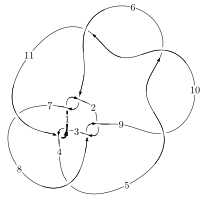
\includegraphics[width=112pt]{../../../GIT/diagram.site/Diagrams/png/570_11a_321.png}\\
\ \ \ A knot diagram\footnotemark}&
\allowdisplaybreaks
\textbf{Linearized knot diagam} \\
\cline{2-2}
 &
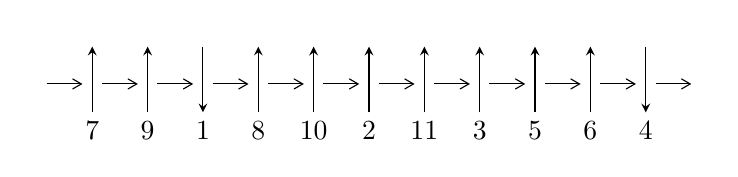
\begin{tikzpicture}[x=20pt, y=17pt]
	% nodes
	\node (C0) at (0, 0) {};
	\node (C1) at (1, 0) {};
	\node (C1U) at (1, +1) {};
	\node (C1D) at (1, -1) {7};

	\node (C2) at (2, 0) {};
	\node (C2U) at (2, +1) {};
	\node (C2D) at (2, -1) {9};

	\node (C3) at (3, 0) {};
	\node (C3U) at (3, +1) {};
	\node (C3D) at (3, -1) {1};

	\node (C4) at (4, 0) {};
	\node (C4U) at (4, +1) {};
	\node (C4D) at (4, -1) {8};

	\node (C5) at (5, 0) {};
	\node (C5U) at (5, +1) {};
	\node (C5D) at (5, -1) {10};

	\node (C6) at (6, 0) {};
	\node (C6U) at (6, +1) {};
	\node (C6D) at (6, -1) {2};

	\node (C7) at (7, 0) {};
	\node (C7U) at (7, +1) {};
	\node (C7D) at (7, -1) {11};

	\node (C8) at (8, 0) {};
	\node (C8U) at (8, +1) {};
	\node (C8D) at (8, -1) {3};

	\node (C9) at (9, 0) {};
	\node (C9U) at (9, +1) {};
	\node (C9D) at (9, -1) {5};

	\node (C10) at (10, 0) {};
	\node (C10U) at (10, +1) {};
	\node (C10D) at (10, -1) {6};

	\node (C11) at (11, 0) {};
	\node (C11U) at (11, +1) {};
	\node (C11D) at (11, -1) {4};
	\node (C12) at (12, 0) {};

	% arrows
	\draw[->,>={angle 60}]
	(C0) edge (C1) (C1) edge (C2) (C2) edge (C3) (C3) edge (C4) (C4) edge (C5) (C5) edge (C6) (C6) edge (C7) (C7) edge (C8) (C8) edge (C9) (C9) edge (C10) (C10) edge (C11) (C11) edge (C12) ;	\draw[->,>=stealth]
	(C1D) edge (C1U) (C2D) edge (C2U) (C3U) edge (C3D) (C4D) edge (C4U) (C5D) edge (C5U) (C6D) edge (C6U) (C7D) edge (C7U) (C8D) edge (C8U) (C9D) edge (C9U) (C10D) edge (C10U) (C11U) edge (C11D) ;
	\end{tikzpicture} \\
\hhline{~~} \\& 
\textbf{Solving Sequence} \\ \cline{2-2} 
 &
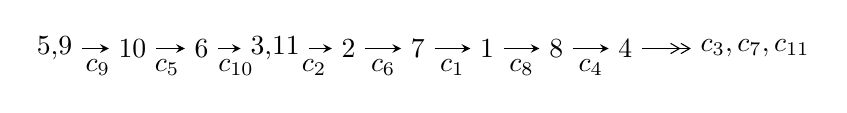
\begin{tikzpicture}[x=25pt, y=7pt]
	% node
	\node (A0) at (-1/8, 0) {5,9};
	\node (A1) at (1, 0) {10};
	\node (A2) at (2, 0) {6};
	\node (A3) at (49/16, 0) {3,11};
	\node (A4) at (33/8, 0) {2};
	\node (A5) at (41/8, 0) {7};
	\node (A6) at (49/8, 0) {1};
	\node (A7) at (57/8, 0) {8};
	\node (A8) at (65/8, 0) {4};
	\node (C1) at (1/2, -1) {$c_{9}$};
	\node (C2) at (3/2, -1) {$c_{5}$};
	\node (C3) at (5/2, -1) {$c_{10}$};
	\node (C4) at (29/8, -1) {$c_{2}$};
	\node (C5) at (37/8, -1) {$c_{6}$};
	\node (C6) at (45/8, -1) {$c_{1}$};
	\node (C7) at (53/8, -1) {$c_{8}$};
	\node (C8) at (61/8, -1) {$c_{4}$};
	\node (A9) at (10, 0) {$c_{3},c_{7},c_{11}$};

	% edge
	\draw[->,>=stealth]	
	(A0) edge (A1) (A1) edge (A2) (A2) edge (A3) (A3) edge (A4) (A4) edge (A5) (A5) edge (A6) (A6) edge (A7) (A7) edge (A8) ;
	\draw[->>,>={angle 60}]	
	(A8) edge (A9);
\end{tikzpicture} \\ 

\end{tabular} \\

\footnotetext{
The image of knot diagram is generated by the software ``\textbf{Draw programme}" developed by Andrew Bartholomew(\url{http://www.layer8.co.uk/maths/draw/index.htm\#Running-draw}), where we modified some parts for our purpose(\url{https://github.com/CATsTAILs/LinksPainter}).
}\phantom \\ \newline 
\centering \textbf{Ideals for irreducible components\footnotemark of $X_{\text{par}}$} 
 
\begin{align*}
I^u_{1}&=\langle 
1073 u^{25}+10099 u^{24}+\cdots+16 b-21648,\;-299 u^{25}-2899 u^{24}+\cdots+32 a+7504,\\
\phantom{I^u_{1}}&\phantom{= \langle  }u^{26}+11 u^{25}+\cdots+16 u-32\rangle \\
I^u_{2}&=\langle 
u^3 a+u^4- u^3- a u- u^2+b- a,\;u^3 a- u^4+2 u^3+a^2- a u+2 u^2-2 a-4 u,\;u^5- u^4-2 u^3+u^2+u+1\rangle \\
I^u_{3}&=\langle 
-325652548336533 a^7 u^4-216522091497175 a^6 u^4+\cdots+461842568426094 a-37300538969198,\\
\phantom{I^u_{3}}&\phantom{= \langle  }2 a^7 u^4+3 a^6 u^4+\cdots+63 a+36,\;u^5- u^4-2 u^3+u^2+u+1\rangle \\
I^u_{4}&=\langle 
u^{15}-2 u^{14}-8 u^{13}+16 u^{12}+23 u^{11}-49 u^{10}-30 u^9+74 u^8+21 u^7-63 u^6-11 u^5+33 u^4+3 u^3-9 u^2+b+2,\\
\phantom{I^u_{4}}&\phantom{= \langle  }- u^{14}+u^{13}+8 u^{12}-8 u^{11}-24 u^{10}+24 u^9+36 u^8-34 u^7-34 u^6+25 u^5+24 u^4-9 u^3-10 u^2+a+3,\\
\phantom{I^u_{4}}&\phantom{= \langle  }u^{16}-9 u^{14}+u^{13}+33 u^{12}-6 u^{11}-64 u^{10}+13 u^9+73 u^8-12 u^7-52 u^6+4 u^5+22 u^4-4 u^2+1\rangle \\
\\
\end{align*}
\raggedright * 4 irreducible components of $\dim_{\mathbb{C}}=0$, with total 92 representations.\\
\footnotetext{All coefficients of polynomials are rational numbers. But the coefficients are sometimes approximated in decimal forms when there is not enough margin.}
\newpage
\renewcommand{\arraystretch}{1}
\centering \section*{I. $I^u_{1}= \langle 1073 u^{25}+10099 u^{24}+\cdots+16 b-21648,\;-299 u^{25}-2899 u^{24}+\cdots+32 a+7504,\;u^{26}+11 u^{25}+\cdots+16 u-32 \rangle$}
\flushleft \textbf{(i) Arc colorings}\\
\begin{tabular}{m{7pt} m{180pt} m{7pt} m{180pt} }
\flushright $a_{5}=$&$\begin{pmatrix}0\\u\end{pmatrix}$ \\
\flushright $a_{9}=$&$\begin{pmatrix}1\\0\end{pmatrix}$ \\
\flushright $a_{10}=$&$\begin{pmatrix}1\\- u^2\end{pmatrix}$ \\
\flushright $a_{6}=$&$\begin{pmatrix}u\\- u^3+u\end{pmatrix}$ \\
\flushright $a_{3}=$&$\begin{pmatrix}\frac{299}{32} u^{25}+\frac{2899}{32} u^{24}+\cdots+301 u-\frac{469}{2}\\-67.0625 u^{25}-631.188 u^{24}+\cdots-1534 u+1353\end{pmatrix}$ \\
\flushright $a_{11}=$&$\begin{pmatrix}- u^2+1\\u^4-2 u^2\end{pmatrix}$ \\
\flushright $a_{2}=$&$\begin{pmatrix}\frac{2445}{32} u^{25}+\frac{23097}{32} u^{24}+\cdots+1835 u-\frac{3175}{2}\\-67.0625 u^{25}-631.188 u^{24}+\cdots-1534 u+1353\end{pmatrix}$ \\
\flushright $a_{7}=$&$\begin{pmatrix}-13.7500 u^{25}-133.250 u^{24}+\cdots-383.500 u+320.500\\4 u^{25}+42 u^{24}+\cdots+\frac{377}{2} u-136\end{pmatrix}$ \\
\flushright $a_{1}=$&$\begin{pmatrix}\frac{1181}{16} u^{25}+\frac{5595}{8} u^{24}+\cdots+1708 u-1515\\\frac{107}{16} u^{25}+\frac{871}{16} u^{24}+\cdots-43 u-22\end{pmatrix}$ \\
\flushright $a_{8}=$&$\begin{pmatrix}\frac{39}{4} u^{25}+\frac{365}{4} u^{24}+\cdots+197 u-\frac{367}{2}\\-4 u^{25}-42 u^{24}+\cdots-\frac{375}{2} u+136\end{pmatrix}$ \\
\flushright $a_{4}=$&$\begin{pmatrix}\frac{5}{4} u^{25}+\frac{75}{4} u^{24}+\cdots+\frac{863}{4} u-128\\\frac{185}{4} u^{25}+\frac{891}{2} u^{24}+\cdots+1245 u-1048\end{pmatrix}$\\ \flushright $a_{4}=$&$\begin{pmatrix}\frac{5}{4} u^{25}+\frac{75}{4} u^{24}+\cdots+\frac{863}{4} u-128\\\frac{185}{4} u^{25}+\frac{891}{2} u^{24}+\cdots+1245 u-1048\end{pmatrix}$\\&\end{tabular}
\flushleft \textbf{(ii) Obstruction class $= -1$}\\~\\
\flushleft \textbf{(iii) Cusp Shapes $= \frac{333}{2} u^{25}+1571 u^{24}+\cdots+3724 u-3326$}\\~\\
\newpage\renewcommand{\arraystretch}{1}
\flushleft \textbf{(iv) u-Polynomials at the component}\newline \\
\begin{tabular}{m{50pt}|m{274pt}}
Crossings & \hspace{64pt}u-Polynomials at each crossing \\
\hline $$\begin{aligned}c_{1},c_{2},c_{6}\\c_{8}\end{aligned}$$&$\begin{aligned}
&u^{26}+7 u^{24}+\cdots+3 u-1
\end{aligned}$\\
\hline $$\begin{aligned}c_{3},c_{11}\end{aligned}$$&$\begin{aligned}
&u^{26}-12 u^{25}+\cdots-448 u+32
\end{aligned}$\\
\hline $$\begin{aligned}c_{4},c_{7}\end{aligned}$$&$\begin{aligned}
&u^{26}-9 u^{24}+\cdots-16 u^2-1
\end{aligned}$\\
\hline $$\begin{aligned}c_{5},c_{9},c_{10}\end{aligned}$$&$\begin{aligned}
&u^{26}+11 u^{25}+\cdots+16 u-32
\end{aligned}$\\
\hline
\end{tabular}\\~\\
\newpage\renewcommand{\arraystretch}{1}
\flushleft \textbf{(v) Riley Polynomials at the component}\newline \\
\begin{tabular}{m{50pt}|m{274pt}}
Crossings & \hspace{64pt}Riley Polynomials at each crossing \\
\hline $$\begin{aligned}c_{1},c_{2},c_{6}\\c_{8}\end{aligned}$$&$\begin{aligned}
&y^{26}+14 y^{25}+\cdots- y+1
\end{aligned}$\\
\hline $$\begin{aligned}c_{3},c_{11}\end{aligned}$$&$\begin{aligned}
&y^{26}+10 y^{25}+\cdots-27136 y+1024
\end{aligned}$\\
\hline $$\begin{aligned}c_{4},c_{7}\end{aligned}$$&$\begin{aligned}
&y^{26}-18 y^{25}+\cdots+32 y+1
\end{aligned}$\\
\hline $$\begin{aligned}c_{5},c_{9},c_{10}\end{aligned}$$&$\begin{aligned}
&y^{26}-23 y^{25}+\cdots-5888 y+1024
\end{aligned}$\\
\hline
\end{tabular}\\~\\
\newpage\flushleft \textbf{(vi) Complex Volumes and Cusp Shapes}
$$\begin{array}{c|c|c}  
\text{Solutions to }I^u_{1}& \I (\text{vol} + \sqrt{-1}CS) & \text{Cusp shape}\\
 \hline 
\begin{aligned}
u &= \phantom{-}0.383322 + 0.913347 I \\
a &= \phantom{-}0.15913 - 1.78657 I \\
b &= -0.55889 - 1.30495 I\end{aligned}
 & -2.65503 + 11.68360 I & \phantom{-}5.29865 - 8.17521 I \\ \hline\begin{aligned}
u &= \phantom{-}0.383322 - 0.913347 I \\
a &= \phantom{-}0.15913 + 1.78657 I \\
b &= -0.55889 + 1.30495 I\end{aligned}
 & -2.65503 - 11.68360 I & \phantom{-}5.29865 + 8.17521 I \\ \hline\begin{aligned}
u &= -0.828242 + 0.616056 I \\
a &= \phantom{-}0.43855 + 1.53930 I \\
b &= -0.081709 + 0.666053 I\end{aligned}
 & -1.85940 - 2.41843 I & \phantom{-}9.7124 + 14.3057 I \\ \hline\begin{aligned}
u &= -0.828242 - 0.616056 I \\
a &= \phantom{-}0.43855 - 1.53930 I \\
b &= -0.081709 - 0.666053 I\end{aligned}
 & -1.85940 + 2.41843 I & \phantom{-}9.7124 - 14.3057 I \\ \hline\begin{aligned}
u &= \phantom{-}0.317740 + 0.989994 I \\
a &= -0.13580 + 1.61988 I \\
b &= \phantom{-}0.424496 + 1.163430 I\end{aligned}
 & -5.41034 + 5.29072 I & \phantom{-}3.13484 - 6.09748 I \\ \hline\begin{aligned}
u &= \phantom{-}0.317740 - 0.989994 I \\
a &= -0.13580 - 1.61988 I \\
b &= \phantom{-}0.424496 - 1.163430 I\end{aligned}
 & -5.41034 - 5.29072 I & \phantom{-}3.13484 + 6.09748 I \\ \hline\begin{aligned}
u &= \phantom{-}0.867391 + 0.763321 I \\
a &= \phantom{-}0.748452 - 0.780722 I \\
b &= \phantom{-}0.380945 - 1.145790 I\end{aligned}
 & -1.25182 - 6.02050 I & \phantom{-}5.93358 + 4.78066 I \\ \hline\begin{aligned}
u &= \phantom{-}0.867391 - 0.763321 I \\
a &= \phantom{-}0.748452 + 0.780722 I \\
b &= \phantom{-}0.380945 + 1.145790 I\end{aligned}
 & -1.25182 + 6.02050 I & \phantom{-}5.93358 - 4.78066 I \\ \hline\begin{aligned}
u &= \phantom{-}0.604803 + 0.424043 I \\
a &= \phantom{-}0.576639 + 0.245391 I \\
b &= \phantom{-}0.695203 - 0.396515 I\end{aligned}
 & \phantom{-}3.26437 + 1.57845 I & \phantom{-}12.40306 - 2.05363 I \\ \hline\begin{aligned}
u &= \phantom{-}0.604803 - 0.424043 I \\
a &= \phantom{-}0.576639 - 0.245391 I \\
b &= \phantom{-}0.695203 + 0.396515 I\end{aligned}
 & \phantom{-}3.26437 - 1.57845 I & \phantom{-}12.40306 + 2.05363 I\\
 \hline 
 \end{array}$$\newpage$$\begin{array}{c|c|c}  
\text{Solutions to }I^u_{1}& \I (\text{vol} + \sqrt{-1}CS) & \text{Cusp shape}\\
 \hline 
\begin{aligned}
u &= \phantom{-}0.155329 + 0.682857 I \\
a &= -0.12123 - 1.47536 I \\
b &= -0.595161 - 0.658480 I\end{aligned}
 & \phantom{-}1.79534 + 1.92657 I & \phantom{-}9.32234 - 4.27733 I \\ \hline\begin{aligned}
u &= \phantom{-}0.155329 - 0.682857 I \\
a &= -0.12123 + 1.47536 I \\
b &= -0.595161 + 0.658480 I\end{aligned}
 & \phantom{-}1.79534 - 1.92657 I & \phantom{-}9.32234 + 4.27733 I \\ \hline\begin{aligned}
u &= \phantom{-}1.081110 + 0.752925 I \\
a &= -0.476440 + 0.754455 I \\
b &= -0.236698 + 1.023340 I\end{aligned}
 & -3.21650 + 0.73193 I & \phantom{-}6.23274 + 2.78423 I \\ \hline\begin{aligned}
u &= \phantom{-}1.081110 - 0.752925 I \\
a &= -0.476440 - 0.754455 I \\
b &= -0.236698 - 1.023340 I\end{aligned}
 & -3.21650 - 0.73193 I & \phantom{-}6.23274 - 2.78423 I \\ \hline\begin{aligned}
u &= -1.37365 + 0.35020 I \\
a &= -0.829144 - 1.069810 I \\
b &= \phantom{-}0.726167 - 0.875974 I\end{aligned}
 & \phantom{-}6.54594 - 5.84781 I & \phantom{-}12.9077 + 6.2870 I \\ \hline\begin{aligned}
u &= -1.37365 - 0.35020 I \\
a &= -0.829144 + 1.069810 I \\
b &= \phantom{-}0.726167 + 0.875974 I\end{aligned}
 & \phantom{-}6.54594 + 5.84781 I & \phantom{-}12.9077 - 6.2870 I \\ \hline\begin{aligned}
u &= -1.47715\phantom{ +0.000000I} \\
a &= -0.340449\phantom{ +0.000000I} \\
b &= \phantom{-}0.812944\phantom{ +0.000000I}\end{aligned}
 & \phantom{-}7.01191\phantom{ +0.000000I} & \phantom{-}13.1000\phantom{ +0.000000I} \\ \hline\begin{aligned}
u &= -1.51143 + 0.09637 I \\
a &= \phantom{-}0.142803 + 0.338489 I \\
b &= -0.920008 - 0.217229 I\end{aligned}
 & \phantom{-}10.23750 - 3.38664 I & \phantom{-}16.0962 + 0. I\phantom{ +0.000000I} \\ \hline\begin{aligned}
u &= -1.51143 - 0.09637 I \\
a &= \phantom{-}0.142803 - 0.338489 I \\
b &= -0.920008 + 0.217229 I\end{aligned}
 & \phantom{-}10.23750 + 3.38664 I & \phantom{-}16.0962 + 0. I\phantom{ +0.000000I} \\ \hline\begin{aligned}
u &= -1.47229 + 0.38599 I \\
a &= \phantom{-}0.852447 + 0.991797 I \\
b &= -0.618131 + 1.238700 I\end{aligned}
 & \phantom{-}0.31031 - 10.20530 I & \phantom{-}7.00000 + 6.34949 I\\
 \hline 
 \end{array}$$\newpage$$\begin{array}{c|c|c}  
\text{Solutions to }I^u_{1}& \I (\text{vol} + \sqrt{-1}CS) & \text{Cusp shape}\\
 \hline 
\begin{aligned}
u &= -1.47229 - 0.38599 I \\
a &= \phantom{-}0.852447 - 0.991797 I \\
b &= -0.618131 - 1.238700 I\end{aligned}
 & \phantom{-}0.31031 + 10.20530 I & \phantom{-}7.00000 - 6.34949 I \\ \hline\begin{aligned}
u &= -1.48560 + 0.35379 I \\
a &= -0.921287 - 1.008460 I \\
b &= \phantom{-}0.73457 - 1.37086 I\end{aligned}
 & \phantom{-}3.3294 - 16.2583 I & \phantom{-0.000000 -}0. + 8.72442 I \\ \hline\begin{aligned}
u &= -1.48560 - 0.35379 I \\
a &= -0.921287 + 1.008460 I \\
b &= \phantom{-}0.73457 + 1.37086 I\end{aligned}
 & \phantom{-}3.3294 + 16.2583 I & \phantom{-0.000000 } 0. - 8.72442 I \\ \hline\begin{aligned}
u &= \phantom{-}0.423114\phantom{ +0.000000I} \\
a &= \phantom{-}0.218860\phantom{ +0.000000I} \\
b &= -0.331232\phantom{ +0.000000I}\end{aligned}
 & \phantom{-}0.617191\phantom{ +0.000000I} & \phantom{-}16.1820\phantom{ +0.000000I} \\ \hline\begin{aligned}
u &= -1.71146 + 0.07064 I \\
a &= -0.123322 - 0.123466 I \\
b &= -0.191640 - 0.759101 I\end{aligned}
 & \phantom{-}8.12481 + 2.87714 I & \phantom{-0.000000 } 0 \\ \hline\begin{aligned}
u &= -1.71146 - 0.07064 I \\
a &= -0.123322 + 0.123466 I \\
b &= -0.191640 + 0.759101 I\end{aligned}
 & \phantom{-}8.12481 - 2.87714 I & \phantom{-0.000000 } 0\\
 \hline 
 \end{array}$$\newpage\newpage\renewcommand{\arraystretch}{1}
\centering \section*{II. $I^u_{2}= \langle u^3 a+u^4- u^3- a u- u^2+b- a,\;u^3 a- u^4+2 u^3+a^2- a u+2 u^2-2 a-4 u,\;u^5- u^4-2 u^3+u^2+u+1 \rangle$}
\flushleft \textbf{(i) Arc colorings}\\
\begin{tabular}{m{7pt} m{180pt} m{7pt} m{180pt} }
\flushright $a_{5}=$&$\begin{pmatrix}0\\u\end{pmatrix}$ \\
\flushright $a_{9}=$&$\begin{pmatrix}1\\0\end{pmatrix}$ \\
\flushright $a_{10}=$&$\begin{pmatrix}1\\- u^2\end{pmatrix}$ \\
\flushright $a_{6}=$&$\begin{pmatrix}u\\- u^3+u\end{pmatrix}$ \\
\flushright $a_{3}=$&$\begin{pmatrix}a\\- u^3 a- u^4+u^3+a u+u^2+a\end{pmatrix}$ \\
\flushright $a_{11}=$&$\begin{pmatrix}- u^2+1\\u^4-2 u^2\end{pmatrix}$ \\
\flushright $a_{2}=$&$\begin{pmatrix}u^3 a+u^4- u^3- a u- u^2\\- u^3 a- u^4+u^3+a u+u^2+a\end{pmatrix}$ \\
\flushright $a_{7}=$&$\begin{pmatrix}u^4 a- u^3 a- u^2 a- u^3- u^2+3 u\\u^2-2\end{pmatrix}$ \\
\flushright $a_{1}=$&$\begin{pmatrix}- u^4+u^2 a+u^3+u^2- a- u+1\\- u^4 a+2 u^2 a- u^2+u+1\end{pmatrix}$ \\
\flushright $a_{8}=$&$\begin{pmatrix}- u^3 a+a u+a+u-1\\- u^4- u^2 a+3 u^2-1\end{pmatrix}$ \\
\flushright $a_{4}=$&$\begin{pmatrix}- u^3 a- u^4+2 a u+2 u^2-1\\- a- u\end{pmatrix}$\\ \flushright $a_{4}=$&$\begin{pmatrix}- u^3 a- u^4+2 a u+2 u^2-1\\- a- u\end{pmatrix}$\\&\end{tabular}
\flushleft \textbf{(ii) Obstruction class $= -1$}\\~\\
\flushleft \textbf{(iii) Cusp Shapes $= -8 u^3+16 u+10$}\\~\\
\newpage\renewcommand{\arraystretch}{1}
\flushleft \textbf{(iv) u-Polynomials at the component}\newline \\
\begin{tabular}{m{50pt}|m{274pt}}
Crossings & \hspace{64pt}u-Polynomials at each crossing \\
\hline $$\begin{aligned}c_{1},c_{2},c_{6}\\c_{8}\end{aligned}$$&$\begin{aligned}
&u^{10}+2 u^9+\cdots+8 u+17
\end{aligned}$\\
\hline $$\begin{aligned}c_{3},c_{11}\end{aligned}$$&$\begin{aligned}
&(u^5+u^4+2 u^3+u^2+u+1)^2
\end{aligned}$\\
\hline $$\begin{aligned}c_{4},c_{7}\end{aligned}$$&$\begin{aligned}
&u^{10}+2 u^9+3 u^8+4 u^6+15 u^4-16 u^3+33 u^2-20 u+7
\end{aligned}$\\
\hline $$\begin{aligned}c_{5},c_{9},c_{10}\end{aligned}$$&$\begin{aligned}
&(u^5- u^4-2 u^3+u^2+u+1)^2
\end{aligned}$\\
\hline
\end{tabular}\\~\\
\newpage\renewcommand{\arraystretch}{1}
\flushleft \textbf{(v) Riley Polynomials at the component}\newline \\
\begin{tabular}{m{50pt}|m{274pt}}
Crossings & \hspace{64pt}Riley Polynomials at each crossing \\
\hline $$\begin{aligned}c_{1},c_{2},c_{6}\\c_{8}\end{aligned}$$&$\begin{aligned}
&y^{10}+6 y^9+\cdots+786 y+289
\end{aligned}$\\
\hline $$\begin{aligned}c_{3},c_{11}\end{aligned}$$&$\begin{aligned}
&(y^5+3 y^4+4 y^3+y^2- y-1)^2
\end{aligned}$\\
\hline $$\begin{aligned}c_{4},c_{7}\end{aligned}$$&$\begin{aligned}
&y^{10}+2 y^9+\cdots+62 y+49
\end{aligned}$\\
\hline $$\begin{aligned}c_{5},c_{9},c_{10}\end{aligned}$$&$\begin{aligned}
&(y^5-5 y^4+8 y^3-3 y^2- y-1)^2
\end{aligned}$\\
\hline
\end{tabular}\\~\\
\newpage\flushleft \textbf{(vi) Complex Volumes and Cusp Shapes}
$$\begin{array}{c|c|c}  
\text{Solutions to }I^u_{2}& \I (\text{vol} + \sqrt{-1}CS) & \text{Cusp shape}\\
 \hline 
\begin{aligned}
u &= -1.21774\phantom{ +0.000000I} \\
a &= \phantom{-}1.29401 + 0.59312 I \\
b &= -0.466896 + 0.941886 I\end{aligned}
 & -0.132640\phantom{ +0.000000I} & \phantom{-}4.96230\phantom{ +0.000000I} \\ \hline\begin{aligned}
u &= -1.21774\phantom{ +0.000000I} \\
a &= \phantom{-}1.29401 - 0.59312 I \\
b &= -0.466896 - 0.941886 I\end{aligned}
 & -0.132640\phantom{ +0.000000I} & \phantom{-}4.96230\phantom{ +0.000000I} \\ \hline\begin{aligned}
u &= -0.309916 + 0.549911 I \\
a &= -0.422523 - 1.226950 I \\
b &= \phantom{-}0.617609 - 1.263280 I\end{aligned}
 & -4.27660 - 3.06116 I & \phantom{-}3.03023 + 8.86130 I \\ \hline\begin{aligned}
u &= -0.309916 + 0.549911 I \\
a &= \phantom{-}1.86122 + 1.78470 I \\
b &= -0.060281 + 1.331670 I\end{aligned}
 & -4.27660 - 3.06116 I & \phantom{-}3.03023 + 8.86130 I \\ \hline\begin{aligned}
u &= -0.309916 - 0.549911 I \\
a &= -0.422523 + 1.226950 I \\
b &= \phantom{-}0.617609 + 1.263280 I\end{aligned}
 & -4.27660 + 3.06116 I & \phantom{-}3.03023 - 8.86130 I \\ \hline\begin{aligned}
u &= -0.309916 - 0.549911 I \\
a &= \phantom{-}1.86122 - 1.78470 I \\
b &= -0.060281 - 1.331670 I\end{aligned}
 & -4.27660 + 3.06116 I & \phantom{-}3.03023 - 8.86130 I \\ \hline\begin{aligned}
u &= \phantom{-}1.41878 + 0.21917 I \\
a &= \phantom{-}1.00071 - 1.33190 I \\
b &= -0.547449 - 1.293710 I\end{aligned}
 & \phantom{-}6.81032 + 8.80167 I & \phantom{-}11.48863 - 6.99717 I \\ \hline\begin{aligned}
u &= \phantom{-}1.41878 + 0.21917 I \\
a &= -0.233411 + 0.238092 I \\
b &= \phantom{-}1.45702 - 0.30917 I\end{aligned}
 & \phantom{-}6.81032 + 8.80167 I & \phantom{-}11.48863 - 6.99717 I \\ \hline\begin{aligned}
u &= \phantom{-}1.41878 - 0.21917 I \\
a &= \phantom{-}1.00071 + 1.33190 I \\
b &= -0.547449 + 1.293710 I\end{aligned}
 & \phantom{-}6.81032 - 8.80167 I & \phantom{-}11.48863 + 6.99717 I \\ \hline\begin{aligned}
u &= \phantom{-}1.41878 - 0.21917 I \\
a &= -0.233411 - 0.238092 I \\
b &= \phantom{-}1.45702 + 0.30917 I\end{aligned}
 & \phantom{-}6.81032 - 8.80167 I & \phantom{-}11.48863 + 6.99717 I\\
 \hline 
 \end{array}$$\newpage\newpage\renewcommand{\arraystretch}{1}
\centering \section*{III. $I^u_{3}= \langle -3.26\times10^{14} a^{7} u^{4}-2.17\times10^{14} a^{6} u^{4}+\cdots+4.62\times10^{14} a-3.73\times10^{13},\;2 a^7 u^4+3 a^6 u^4+\cdots+63 a+36,\;u^5- u^4-2 u^3+u^2+u+1 \rangle$}
\flushleft \textbf{(i) Arc colorings}\\
\begin{tabular}{m{7pt} m{180pt} m{7pt} m{180pt} }
\flushright $a_{5}=$&$\begin{pmatrix}0\\u\end{pmatrix}$ \\
\flushright $a_{9}=$&$\begin{pmatrix}1\\0\end{pmatrix}$ \\
\flushright $a_{10}=$&$\begin{pmatrix}1\\- u^2\end{pmatrix}$ \\
\flushright $a_{6}=$&$\begin{pmatrix}u\\- u^3+u\end{pmatrix}$ \\
\flushright $a_{3}=$&$\begin{pmatrix}a\\1.78373 a^{7} u^{4}+1.18598 a^{6} u^{4}+\cdots-2.52970 a+0.204311\end{pmatrix}$ \\
\flushright $a_{11}=$&$\begin{pmatrix}- u^2+1\\u^4-2 u^2\end{pmatrix}$ \\
\flushright $a_{2}=$&$\begin{pmatrix}-1.78373 a^{7} u^{4}-1.18598 a^{6} u^{4}+\cdots+3.52970 a-0.204311\\1.78373 a^{7} u^{4}+1.18598 a^{6} u^{4}+\cdots-2.52970 a+0.204311\end{pmatrix}$ \\
\flushright $a_{7}=$&$\begin{pmatrix}-0.513662 a^{7} u^{4}-0.154648 a^{6} u^{4}+\cdots+1.00013 a+0.425409\\0.452703 a^{7} u^{4}+0.296357 a^{6} u^{4}+\cdots-0.697071 a-0.200491\end{pmatrix}$ \\
\flushright $a_{1}=$&$\begin{pmatrix}-0.431150 a^{7} u^{4}-0.236002 a^{6} u^{4}+\cdots+1.67334 a-0.859074\\1.74389 a^{7} u^{4}+0.846631 a^{6} u^{4}+\cdots-3.09895 a+1.01675\end{pmatrix}$ \\
\flushright $a_{8}=$&$\begin{pmatrix}0.158932 a^{7} u^{4}+0.0166854 a^{6} u^{4}+\cdots+0.0570178 a+1.29770\\0.0505083 a^{7} u^{4}-0.709704 a^{6} u^{4}+\cdots+0.671481 a+1.16410\end{pmatrix}$ \\
\flushright $a_{4}=$&$\begin{pmatrix}-0.381857 a^{7} u^{4}+0.0243899 a^{6} u^{4}+\cdots+1.70012 a+0.510808\\-1.20422 a^{7} u^{4}-0.158188 a^{6} u^{4}+\cdots+1.44338 a-0.285170\end{pmatrix}$\\ \flushright $a_{4}=$&$\begin{pmatrix}-0.381857 a^{7} u^{4}+0.0243899 a^{6} u^{4}+\cdots+1.70012 a+0.510808\\-1.20422 a^{7} u^{4}-0.158188 a^{6} u^{4}+\cdots+1.44338 a-0.285170\end{pmatrix}$\\&\end{tabular}
\flushleft \textbf{(ii) Obstruction class $= -1$}\\~\\
\flushleft \textbf{(iii) Cusp Shapes $= \frac{52949256522924}{91283920109957} a^7 u^4+\frac{90213951943262}{91283920109957} a^6 u^4+\cdots+\frac{111428618111312}{91283920109957} a+\frac{970857959574538}{91283920109957}$}\\~\\
\newpage\renewcommand{\arraystretch}{1}
\flushleft \textbf{(iv) u-Polynomials at the component}\newline \\
\begin{tabular}{m{50pt}|m{274pt}}
Crossings & \hspace{64pt}u-Polynomials at each crossing \\
\hline $$\begin{aligned}c_{1},c_{2},c_{6}\\c_{8}\end{aligned}$$&$\begin{aligned}
&u^{40}- u^{39}+\cdots+112 u+32
\end{aligned}$\\
\hline $$\begin{aligned}c_{3},c_{11}\end{aligned}$$&$\begin{aligned}
&(u^5+u^4+2 u^3+u^2+u+1)^8
\end{aligned}$\\
\hline $$\begin{aligned}c_{4},c_{7}\end{aligned}$$&$\begin{aligned}
&u^{40}-7 u^{39}+\cdots+80 u+32
\end{aligned}$\\
\hline $$\begin{aligned}c_{5},c_{9},c_{10}\end{aligned}$$&$\begin{aligned}
&(u^5- u^4-2 u^3+u^2+u+1)^8
\end{aligned}$\\
\hline
\end{tabular}\\~\\
\newpage\renewcommand{\arraystretch}{1}
\flushleft \textbf{(v) Riley Polynomials at the component}\newline \\
\begin{tabular}{m{50pt}|m{274pt}}
Crossings & \hspace{64pt}Riley Polynomials at each crossing \\
\hline $$\begin{aligned}c_{1},c_{2},c_{6}\\c_{8}\end{aligned}$$&$\begin{aligned}
&y^{40}+29 y^{39}+\cdots+8960 y+1024
\end{aligned}$\\
\hline $$\begin{aligned}c_{3},c_{11}\end{aligned}$$&$\begin{aligned}
&(y^5+3 y^4+4 y^3+y^2- y-1)^8
\end{aligned}$\\
\hline $$\begin{aligned}c_{4},c_{7}\end{aligned}$$&$\begin{aligned}
&y^{40}+5 y^{39}+\cdots+9984 y+1024
\end{aligned}$\\
\hline $$\begin{aligned}c_{5},c_{9},c_{10}\end{aligned}$$&$\begin{aligned}
&(y^5-5 y^4+8 y^3-3 y^2- y-1)^8
\end{aligned}$\\
\hline
\end{tabular}\\~\\
\newpage\flushleft \textbf{(vi) Complex Volumes and Cusp Shapes}
$$\begin{array}{c|c|c}  
\text{Solutions to }I^u_{3}& \I (\text{vol} + \sqrt{-1}CS) & \text{Cusp shape}\\
 \hline 
\begin{aligned}
u &= -1.21774\phantom{ +0.000000I} \\
a &= -1.207790 + 0.238764 I \\
b &= \phantom{-}1.020160 + 0.833032 I\end{aligned}
 & \phantom{-}3.33884 + 4.40083 I & \phantom{-}8.22546 - 3.49859 I \\ \hline\begin{aligned}
u &= -1.21774\phantom{ +0.000000I} \\
a &= -1.207790 - 0.238764 I \\
b &= \phantom{-}1.020160 - 0.833032 I\end{aligned}
 & \phantom{-}3.33884 - 4.40083 I & \phantom{-}8.22546 + 3.49859 I \\ \hline\begin{aligned}
u &= -1.21774\phantom{ +0.000000I} \\
a &= \phantom{-}0.256260 + 0.476517 I \\
b &= -0.23486 + 1.89553 I\end{aligned}
 & -2.20462 - 1.53058 I & \phantom{-}3.99626 + 4.43065 I \\ \hline\begin{aligned}
u &= -1.21774\phantom{ +0.000000I} \\
a &= \phantom{-}0.256260 - 0.476517 I \\
b &= -0.23486 - 1.89553 I\end{aligned}
 & -2.20462 + 1.53058 I & \phantom{-}3.99626 - 4.43065 I \\ \hline\begin{aligned}
u &= -1.21774\phantom{ +0.000000I} \\
a &= \phantom{-}0.40240 + 1.64523 I \\
b &= -0.00279 + 1.47385 I\end{aligned}
 & -2.20462 + 1.53058 I & \phantom{-}3.99626 - 4.43065 I \\ \hline\begin{aligned}
u &= -1.21774\phantom{ +0.000000I} \\
a &= \phantom{-}0.40240 - 1.64523 I \\
b &= -0.00279 - 1.47385 I\end{aligned}
 & -2.20462 - 1.53058 I & \phantom{-}3.99626 + 4.43065 I \\ \hline\begin{aligned}
u &= -1.21774\phantom{ +0.000000I} \\
a &= -1.80751 + 0.70455 I \\
b &= \phantom{-}0.067800 + 0.664970 I\end{aligned}
 & \phantom{-}3.33884 - 4.40083 I & \phantom{-}8.22546 + 3.49859 I \\ \hline\begin{aligned}
u &= -1.21774\phantom{ +0.000000I} \\
a &= -1.80751 - 0.70455 I \\
b &= \phantom{-}0.067800 - 0.664970 I\end{aligned}
 & \phantom{-}3.33884 + 4.40083 I & \phantom{-}8.22546 - 3.49859 I \\ \hline\begin{aligned}
u &= -0.309916 + 0.549911 I \\
a &= -0.614210 - 0.356072 I \\
b &= -1.112460 - 0.022805 I\end{aligned}
 & \phantom{-}1.26686 - 5.93141 I & \phantom{-}7.25943 + 7.92923 I \\ \hline\begin{aligned}
u &= -0.309916 + 0.549911 I \\
a &= -0.077663 + 0.645448 I \\
b &= \phantom{-}0.540737 - 0.024289 I\end{aligned}
 & -2.20462 - 1.53058 I & \phantom{-}3.99626 + 4.43065 I\\
 \hline 
 \end{array}$$\newpage$$\begin{array}{c|c|c}  
\text{Solutions to }I^u_{3}& \I (\text{vol} + \sqrt{-1}CS) & \text{Cusp shape}\\
 \hline 
\begin{aligned}
u &= -0.309916 + 0.549911 I \\
a &= -0.69063 - 1.44845 I \\
b &= -0.631776 - 0.881136 I\end{aligned}
 & \phantom{-}1.26686 + 2.87025 I & \phantom{-}7.25943 + 0.93206 I \\ \hline\begin{aligned}
u &= -0.309916 + 0.549911 I \\
a &= \phantom{-}0.72433 + 1.72452 I \\
b &= -0.28691 + 1.51546 I\end{aligned}
 & -4.27660\phantom{ +0.000000I} & \phantom{-}3.03023 + 0. I\phantom{ +0.000000I} \\ \hline\begin{aligned}
u &= -0.309916 + 0.549911 I \\
a &= -1.94655 - 0.78265 I \\
b &= -0.060228 - 1.074110 I\end{aligned}
 & -4.27660\phantom{ +0.000000I} & \phantom{-}3.03023 + 0. I\phantom{ +0.000000I} \\ \hline\begin{aligned}
u &= -0.309916 + 0.549911 I \\
a &= \phantom{-}0.72536 - 2.06070 I \\
b &= \phantom{-}0.330888 - 0.359958 I\end{aligned}
 & \phantom{-}1.26686 + 2.87025 I & \phantom{-}7.25943 + 0.93206 I \\ \hline\begin{aligned}
u &= -0.309916 + 0.549911 I \\
a &= \phantom{-}0.50296 + 2.30075 I \\
b &= -0.127790 + 1.025730 I\end{aligned}
 & -2.20462 - 1.53058 I & \phantom{-}3.99626 + 4.43065 I \\ \hline\begin{aligned}
u &= -0.309916 + 0.549911 I \\
a &= -0.41156 - 2.99999 I \\
b &= \phantom{-}0.451097 - 1.069650 I\end{aligned}
 & \phantom{-}1.26686 - 5.93141 I & \phantom{-}7.25943 + 7.92923 I \\ \hline\begin{aligned}
u &= -0.309916 - 0.549911 I \\
a &= -0.614210 + 0.356072 I \\
b &= -1.112460 + 0.022805 I\end{aligned}
 & \phantom{-}1.26686 + 5.93141 I & \phantom{-}7.25943 - 7.92923 I \\ \hline\begin{aligned}
u &= -0.309916 - 0.549911 I \\
a &= -0.077663 - 0.645448 I \\
b &= \phantom{-}0.540737 + 0.024289 I\end{aligned}
 & -2.20462 + 1.53058 I & \phantom{-}3.99626 - 4.43065 I \\ \hline\begin{aligned}
u &= -0.309916 - 0.549911 I \\
a &= -0.69063 + 1.44845 I \\
b &= -0.631776 + 0.881136 I\end{aligned}
 & \phantom{-}1.26686 - 2.87025 I & \phantom{-}7.25943 - 0.93206 I \\ \hline\begin{aligned}
u &= -0.309916 - 0.549911 I \\
a &= \phantom{-}0.72433 - 1.72452 I \\
b &= -0.28691 - 1.51546 I\end{aligned}
 & -4.27660\phantom{ +0.000000I} & \phantom{-}3.03023 + 0. I\phantom{ +0.000000I}\\
 \hline 
 \end{array}$$\newpage$$\begin{array}{c|c|c}  
\text{Solutions to }I^u_{3}& \I (\text{vol} + \sqrt{-1}CS) & \text{Cusp shape}\\
 \hline 
\begin{aligned}
u &= -0.309916 - 0.549911 I \\
a &= -1.94655 + 0.78265 I \\
b &= -0.060228 + 1.074110 I\end{aligned}
 & -4.27660\phantom{ +0.000000I} & \phantom{-}3.03023 + 0. I\phantom{ +0.000000I} \\ \hline\begin{aligned}
u &= -0.309916 - 0.549911 I \\
a &= \phantom{-}0.72536 + 2.06070 I \\
b &= \phantom{-}0.330888 + 0.359958 I\end{aligned}
 & \phantom{-}1.26686 - 2.87025 I & \phantom{-}7.25943 - 0.93206 I \\ \hline\begin{aligned}
u &= -0.309916 - 0.549911 I \\
a &= \phantom{-}0.50296 - 2.30075 I \\
b &= -0.127790 - 1.025730 I\end{aligned}
 & -2.20462 + 1.53058 I & \phantom{-}3.99626 - 4.43065 I \\ \hline\begin{aligned}
u &= -0.309916 - 0.549911 I \\
a &= -0.41156 + 2.99999 I \\
b &= \phantom{-}0.451097 + 1.069650 I\end{aligned}
 & \phantom{-}1.26686 + 5.93141 I & \phantom{-}7.25943 - 7.92923 I \\ \hline\begin{aligned}
u &= \phantom{-}1.41878 + 0.21917 I \\
a &= -0.862919 + 0.408494 I \\
b &= \phantom{-}0.68021 + 1.39772 I\end{aligned}
 & \phantom{-}1.26686 + 2.87025 I & \phantom{-}7.25943 + 0.93206 I \\ \hline\begin{aligned}
u &= \phantom{-}1.41878 + 0.21917 I \\
a &= \phantom{-}0.787041 - 0.329401 I \\
b &= -1.02988 - 1.04062 I\end{aligned}
 & \phantom{-}1.26686 + 5.93141 I & \phantom{-}7.25943 - 7.92923 I \\ \hline\begin{aligned}
u &= \phantom{-}1.41878 + 0.21917 I \\
a &= \phantom{-}1.194210 + 0.076658 I \\
b &= -0.161461 - 0.775177 I\end{aligned}
 & \phantom{-}1.26686 + 2.87025 I & \phantom{-}7.25943 + 0.93206 I \\ \hline\begin{aligned}
u &= \phantom{-}1.41878 + 0.21917 I \\
a &= \phantom{-}0.407015 - 1.193670 I \\
b &= -0.464952 - 0.997444 I\end{aligned}
 & \phantom{-}6.81032\phantom{ +0.000000I} & \phantom{-}11.48863 + 0. I\phantom{ +0.000000I} \\ \hline\begin{aligned}
u &= \phantom{-}1.41878 + 0.21917 I \\
a &= -0.808970 + 1.033880 I \\
b &= \phantom{-}0.427482 + 1.218940 I\end{aligned}
 & \phantom{-}3.33884 + 4.40083 I & \phantom{-}8.22546 - 3.49859 I \\ \hline\begin{aligned}
u &= \phantom{-}1.41878 + 0.21917 I \\
a &= -1.37363 + 0.36155 I \\
b &= \phantom{-}0.228681 + 1.161970 I\end{aligned}
 & \phantom{-}1.26686 + 5.93141 I & \phantom{-}7.25943 - 7.92923 I\\
 \hline 
 \end{array}$$\newpage$$\begin{array}{c|c|c}  
\text{Solutions to }I^u_{3}& \I (\text{vol} + \sqrt{-1}CS) & \text{Cusp shape}\\
 \hline 
\begin{aligned}
u &= \phantom{-}1.41878 + 0.21917 I \\
a &= \phantom{-}0.307395 - 0.017583 I \\
b &= -0.982401 + 0.242528 I\end{aligned}
 & \phantom{-}3.33884 + 4.40083 I & \phantom{-}8.22546 - 3.49859 I \\ \hline\begin{aligned}
u &= \phantom{-}1.41878 + 0.21917 I \\
a &= -0.0055411 - 0.0806818 I \\
b &= \phantom{-}0.848456 - 0.805185 I\end{aligned}
 & \phantom{-}6.81032\phantom{ +0.000000I} & \phantom{-}11.48863 + 0. I\phantom{ +0.000000I} \\ \hline\begin{aligned}
u &= \phantom{-}1.41878 - 0.21917 I \\
a &= -0.862919 - 0.408494 I \\
b &= \phantom{-}0.68021 - 1.39772 I\end{aligned}
 & \phantom{-}1.26686 - 2.87025 I & \phantom{-}7.25943 - 0.93206 I \\ \hline\begin{aligned}
u &= \phantom{-}1.41878 - 0.21917 I \\
a &= \phantom{-}0.787041 + 0.329401 I \\
b &= -1.02988 + 1.04062 I\end{aligned}
 & \phantom{-}1.26686 - 5.93141 I & \phantom{-}7.25943 + 7.92923 I \\ \hline\begin{aligned}
u &= \phantom{-}1.41878 - 0.21917 I \\
a &= \phantom{-}1.194210 - 0.076658 I \\
b &= -0.161461 + 0.775177 I\end{aligned}
 & \phantom{-}1.26686 - 2.87025 I & \phantom{-}7.25943 - 0.93206 I \\ \hline\begin{aligned}
u &= \phantom{-}1.41878 - 0.21917 I \\
a &= \phantom{-}0.407015 + 1.193670 I \\
b &= -0.464952 + 0.997444 I\end{aligned}
 & \phantom{-}6.81032\phantom{ +0.000000I} & \phantom{-}11.48863 + 0. I\phantom{ +0.000000I} \\ \hline\begin{aligned}
u &= \phantom{-}1.41878 - 0.21917 I \\
a &= -0.808970 - 1.033880 I \\
b &= \phantom{-}0.427482 - 1.218940 I\end{aligned}
 & \phantom{-}3.33884 - 4.40083 I & \phantom{-}8.22546 + 3.49859 I \\ \hline\begin{aligned}
u &= \phantom{-}1.41878 - 0.21917 I \\
a &= -1.37363 - 0.36155 I \\
b &= \phantom{-}0.228681 - 1.161970 I\end{aligned}
 & \phantom{-}1.26686 - 5.93141 I & \phantom{-}7.25943 + 7.92923 I \\ \hline\begin{aligned}
u &= \phantom{-}1.41878 - 0.21917 I \\
a &= \phantom{-}0.307395 + 0.017583 I \\
b &= -0.982401 - 0.242528 I\end{aligned}
 & \phantom{-}3.33884 - 4.40083 I & \phantom{-}8.22546 + 3.49859 I \\ \hline\begin{aligned}
u &= \phantom{-}1.41878 - 0.21917 I \\
a &= -0.0055411 + 0.0806818 I \\
b &= \phantom{-}0.848456 + 0.805185 I\end{aligned}
 & \phantom{-}6.81032\phantom{ +0.000000I} & \phantom{-}11.48863 + 0. I\phantom{ +0.000000I}\\
 \hline 
 \end{array}$$\newpage\newpage\renewcommand{\arraystretch}{1}
\centering \section*{IV. $I^u_{4}= \langle u^{15}-2 u^{14}+\cdots+b+2,\;- u^{14}+u^{13}+\cdots+a+3,\;u^{16}-9 u^{14}+\cdots-4 u^2+1 \rangle$}
\flushleft \textbf{(i) Arc colorings}\\
\begin{tabular}{m{7pt} m{180pt} m{7pt} m{180pt} }
\flushright $a_{5}=$&$\begin{pmatrix}0\\u\end{pmatrix}$ \\
\flushright $a_{9}=$&$\begin{pmatrix}1\\0\end{pmatrix}$ \\
\flushright $a_{10}=$&$\begin{pmatrix}1\\- u^2\end{pmatrix}$ \\
\flushright $a_{6}=$&$\begin{pmatrix}u\\- u^3+u\end{pmatrix}$ \\
\flushright $a_{3}=$&$\begin{pmatrix}u^{14}- u^{13}+\cdots+10 u^2-3\\- u^{15}+2 u^{14}+\cdots+9 u^2-2\end{pmatrix}$ \\
\flushright $a_{11}=$&$\begin{pmatrix}- u^2+1\\u^4-2 u^2\end{pmatrix}$ \\
\flushright $a_{2}=$&$\begin{pmatrix}u^{15}- u^{14}+\cdots+u^2-1\\- u^{15}+2 u^{14}+\cdots+9 u^2-2\end{pmatrix}$ \\
\flushright $a_{7}=$&$\begin{pmatrix}- u^{14}- u^{13}+\cdots- u+2\\u^{13}-7 u^{11}+\cdots+3 u-1\end{pmatrix}$ \\
\flushright $a_{1}=$&$\begin{pmatrix}u^{15}- u^{14}+\cdots-3 u+1\\2 u^{15}-2 u^{14}+\cdots- u+1\end{pmatrix}$ \\
\flushright $a_{8}=$&$\begin{pmatrix}- u^{14}+8 u^{12}+\cdots-12 u^2+2\\u^{13}-7 u^{11}+\cdots+2 u-1\end{pmatrix}$ \\
\flushright $a_{4}=$&$\begin{pmatrix}- u^{13}+7 u^{11}- u^{10}-18 u^9+4 u^8+21 u^7-4 u^6-12 u^5+2 u^3+u^2+3 u\\- u^{15}+2 u^{14}+\cdots+3 u-2\end{pmatrix}$\\ \flushright $a_{4}=$&$\begin{pmatrix}- u^{13}+7 u^{11}- u^{10}-18 u^9+4 u^8+21 u^7-4 u^6-12 u^5+2 u^3+u^2+3 u\\- u^{15}+2 u^{14}+\cdots+3 u-2\end{pmatrix}$\\&\end{tabular}
\flushleft \textbf{(ii) Obstruction class $= 1$}\\~\\
\flushleft \textbf{(iii) Cusp Shapes $= u^{15}-5 u^{14}-11 u^{13}+38 u^{12}+42 u^{11}-112 u^{10}-77 u^9+161 u^8+82 u^7-122 u^6-63 u^5+48 u^4+28 u^3+2 u+5$}\\~\\
\newpage\renewcommand{\arraystretch}{1}
\flushleft \textbf{(iv) u-Polynomials at the component}\newline \\
\begin{tabular}{m{50pt}|m{274pt}}
Crossings & \hspace{64pt}u-Polynomials at each crossing \\
\hline $$\begin{aligned}c_{1},c_{8}\end{aligned}$$&$\begin{aligned}
&u^{16}+8 u^{14}+\cdots- u+1
\end{aligned}$\\
\hline $$\begin{aligned}c_{2},c_{6}\end{aligned}$$&$\begin{aligned}
&u^{16}+8 u^{14}+\cdots+u+1
\end{aligned}$\\
\hline $$\begin{aligned}c_{3}\end{aligned}$$&$\begin{aligned}
&u^{16}+3 u^{15}+\cdots+5 u^2+1
\end{aligned}$\\
\hline $$\begin{aligned}c_{4},c_{7}\end{aligned}$$&$\begin{aligned}
&u^{16}-3 u^{13}- u^{12}- u^{11}+8 u^8+2 u^7+6 u^6+3 u^5+10 u^4+3 u^2+1
\end{aligned}$\\
\hline $$\begin{aligned}c_{5}\end{aligned}$$&$\begin{aligned}
&u^{16}-9 u^{14}+\cdots-4 u^2+1
\end{aligned}$\\
\hline $$\begin{aligned}c_{9},c_{10}\end{aligned}$$&$\begin{aligned}
&u^{16}-9 u^{14}+\cdots-4 u^2+1
\end{aligned}$\\
\hline $$\begin{aligned}c_{11}\end{aligned}$$&$\begin{aligned}
&u^{16}-3 u^{15}+\cdots+5 u^2+1
\end{aligned}$\\
\hline
\end{tabular}\\~\\
\newpage\renewcommand{\arraystretch}{1}
\flushleft \textbf{(v) Riley Polynomials at the component}\newline \\
\begin{tabular}{m{50pt}|m{274pt}}
Crossings & \hspace{64pt}Riley Polynomials at each crossing \\
\hline $$\begin{aligned}c_{1},c_{2},c_{6}\\c_{8}\end{aligned}$$&$\begin{aligned}
&y^{16}+16 y^{15}+\cdots+13 y+1
\end{aligned}$\\
\hline $$\begin{aligned}c_{3},c_{11}\end{aligned}$$&$\begin{aligned}
&y^{16}+7 y^{15}+\cdots+10 y+1
\end{aligned}$\\
\hline $$\begin{aligned}c_{4},c_{7}\end{aligned}$$&$\begin{aligned}
&y^{16}-2 y^{14}+\cdots+6 y+1
\end{aligned}$\\
\hline $$\begin{aligned}c_{5},c_{9},c_{10}\end{aligned}$$&$\begin{aligned}
&y^{16}-18 y^{15}+\cdots-8 y+1
\end{aligned}$\\
\hline
\end{tabular}\\~\\
\newpage\flushleft \textbf{(vi) Complex Volumes and Cusp Shapes}
$$\begin{array}{c|c|c}  
\text{Solutions to }I^u_{4}& \I (\text{vol} + \sqrt{-1}CS) & \text{Cusp shape}\\
 \hline 
\begin{aligned}
u &= \phantom{-}0.932576 + 0.558604 I \\
a &= \phantom{-}0.83677 - 1.43673 I \\
b &= -0.031814 - 0.697076 I\end{aligned}
 & -2.00312 + 2.11071 I & -0.36261 + 5.84578 I \\ \hline\begin{aligned}
u &= \phantom{-}0.932576 - 0.558604 I \\
a &= \phantom{-}0.83677 + 1.43673 I \\
b &= -0.031814 + 0.697076 I\end{aligned}
 & -2.00312 - 2.11071 I & -0.36261 - 5.84578 I \\ \hline\begin{aligned}
u &= -0.758635 + 0.439917 I \\
a &= -0.543641 - 0.719000 I \\
b &= \phantom{-}0.033972 - 1.283280 I\end{aligned}
 & -4.35479 - 2.08547 I & \phantom{-}2.28739 + 3.71145 I \\ \hline\begin{aligned}
u &= -0.758635 - 0.439917 I \\
a &= -0.543641 + 0.719000 I \\
b &= \phantom{-}0.033972 + 1.283280 I\end{aligned}
 & -4.35479 + 2.08547 I & \phantom{-}2.28739 - 3.71145 I \\ \hline\begin{aligned}
u &= -1.270170 + 0.042100 I \\
a &= -0.117828 - 1.114430 I \\
b &= -0.13344 - 1.70790 I\end{aligned}
 & -1.36561 + 1.03179 I & \phantom{-}13.09233 + 0.83056 I \\ \hline\begin{aligned}
u &= -1.270170 - 0.042100 I \\
a &= -0.117828 + 1.114430 I \\
b &= -0.13344 + 1.70790 I\end{aligned}
 & -1.36561 - 1.03179 I & \phantom{-}13.09233 - 0.83056 I \\ \hline\begin{aligned}
u &= \phantom{-}1.299950 + 0.158892 I \\
a &= -1.49957 + 0.33616 I \\
b &= \phantom{-}0.717514 + 0.694169 I\end{aligned}
 & \phantom{-}4.26074 + 5.75964 I & \phantom{-}11.30648 - 7.65537 I \\ \hline\begin{aligned}
u &= \phantom{-}1.299950 - 0.158892 I \\
a &= -1.49957 - 0.33616 I \\
b &= \phantom{-}0.717514 - 0.694169 I\end{aligned}
 & \phantom{-}4.26074 - 5.75964 I & \phantom{-}11.30648 + 7.65537 I \\ \hline\begin{aligned}
u &= \phantom{-}1.44241 + 0.18942 I \\
a &= \phantom{-}0.942839 - 0.151798 I \\
b &= -0.559613 - 1.118820 I\end{aligned}
 & \phantom{-}1.52375 + 4.32708 I & \phantom{-}9.46348 - 3.89019 I \\ \hline\begin{aligned}
u &= \phantom{-}1.44241 - 0.18942 I \\
a &= \phantom{-}0.942839 + 0.151798 I \\
b &= -0.559613 + 1.118820 I\end{aligned}
 & \phantom{-}1.52375 - 4.32708 I & \phantom{-}9.46348 + 3.89019 I\\
 \hline 
 \end{array}$$\newpage$$\begin{array}{c|c|c}  
\text{Solutions to }I^u_{4}& \I (\text{vol} + \sqrt{-1}CS) & \text{Cusp shape}\\
 \hline 
\begin{aligned}
u &= -0.389768 + 0.361348 I \\
a &= -1.42793 - 0.61604 I \\
b &= \phantom{-}0.199143 - 1.346600 I\end{aligned}
 & -4.35506 - 1.95343 I & \phantom{-}2.10403 + 1.81382 I \\ \hline\begin{aligned}
u &= -0.389768 - 0.361348 I \\
a &= -1.42793 + 0.61604 I \\
b &= \phantom{-}0.199143 + 1.346600 I\end{aligned}
 & -4.35506 + 1.95343 I & \phantom{-}2.10403 - 1.81382 I \\ \hline\begin{aligned}
u &= \phantom{-}0.380311 + 0.321242 I \\
a &= -1.37704 + 2.58113 I \\
b &= -0.462275 + 0.600749 I\end{aligned}
 & \phantom{-}1.00222 - 3.96560 I & \phantom{-}4.29089 + 5.86867 I \\ \hline\begin{aligned}
u &= \phantom{-}0.380311 - 0.321242 I \\
a &= -1.37704 - 2.58113 I \\
b &= -0.462275 - 0.600749 I\end{aligned}
 & \phantom{-}1.00222 + 3.96560 I & \phantom{-}4.29089 - 5.86867 I \\ \hline\begin{aligned}
u &= -1.63668 + 0.04505 I \\
a &= \phantom{-}0.186402 + 0.341093 I \\
b &= \phantom{-}0.236509 + 0.446950 I\end{aligned}
 & \phantom{-}8.58175 + 2.59504 I & \phantom{-}15.8180 + 1.0523 I \\ \hline\begin{aligned}
u &= -1.63668 - 0.04505 I \\
a &= \phantom{-}0.186402 - 0.341093 I \\
b &= \phantom{-}0.236509 - 0.446950 I\end{aligned}
 & \phantom{-}8.58175 - 2.59504 I & \phantom{-}15.8180 - 1.0523 I\\
 \hline 
 \end{array}$$\newpage
\newpage\renewcommand{\arraystretch}{1}
\centering \section*{ V. u-Polynomials}
\begin{tabular}{m{50pt}|m{274pt}}
Crossings & \hspace{64pt}u-Polynomials at each crossing \\
\hline $$\begin{aligned}c_{1},c_{8}\end{aligned}$$&$\begin{aligned}
&(u^{10}+2 u^9+\cdots+8 u+17)(u^{16}+8 u^{14}+\cdots- u+1)\\
&\cdot(u^{26}+7 u^{24}+\cdots+3 u-1)(u^{40}- u^{39}+\cdots+112 u+32)
\end{aligned}$\\
\hline $$\begin{aligned}c_{2},c_{6}\end{aligned}$$&$\begin{aligned}
&(u^{10}+2 u^9+\cdots+8 u+17)(u^{16}+8 u^{14}+\cdots+u+1)\\
&\cdot(u^{26}+7 u^{24}+\cdots+3 u-1)(u^{40}- u^{39}+\cdots+112 u+32)
\end{aligned}$\\
\hline $$\begin{aligned}c_{3}\end{aligned}$$&$\begin{aligned}
&((u^5+u^4+2 u^3+u^2+u+1)^{10})(u^{16}+3 u^{15}+\cdots+5 u^2+1)\\
&\cdot(u^{26}-12 u^{25}+\cdots-448 u+32)
\end{aligned}$\\
\hline $$\begin{aligned}c_{4},c_{7}\end{aligned}$$&$\begin{aligned}
&(u^{10}+2 u^9+3 u^8+4 u^6+15 u^4-16 u^3+33 u^2-20 u+7)\\
&\cdot(u^{16}-3 u^{13}- u^{12}- u^{11}+8 u^8+2 u^7+6 u^6+3 u^5+10 u^4+3 u^2+1)\\
&\cdot(u^{26}-9 u^{24}+\cdots-16 u^2-1)(u^{40}-7 u^{39}+\cdots+80 u+32)
\end{aligned}$\\
\hline $$\begin{aligned}c_{5}\end{aligned}$$&$\begin{aligned}
&((u^5- u^4-2 u^3+u^2+u+1)^{10})(u^{16}-9 u^{14}+\cdots-4 u^2+1)\\
&\cdot(u^{26}+11 u^{25}+\cdots+16 u-32)
\end{aligned}$\\
\hline $$\begin{aligned}c_{9},c_{10}\end{aligned}$$&$\begin{aligned}
&((u^5- u^4-2 u^3+u^2+u+1)^{10})(u^{16}-9 u^{14}+\cdots-4 u^2+1)\\
&\cdot(u^{26}+11 u^{25}+\cdots+16 u-32)
\end{aligned}$\\
\hline $$\begin{aligned}c_{11}\end{aligned}$$&$\begin{aligned}
&((u^5+u^4+2 u^3+u^2+u+1)^{10})(u^{16}-3 u^{15}+\cdots+5 u^2+1)\\
&\cdot(u^{26}-12 u^{25}+\cdots-448 u+32)
\end{aligned}$\\
\hline
\end{tabular}\newpage\renewcommand{\arraystretch}{1}
\centering \section*{ VI. Riley Polynomials}
\begin{tabular}{m{50pt}|m{274pt}}
Crossings & \hspace{64pt}Riley Polynomials at each crossing \\
\hline $$\begin{aligned}c_{1},c_{2},c_{6}\\c_{8}\end{aligned}$$&$\begin{aligned}
&(y^{10}+6 y^9+\cdots+786 y+289)(y^{16}+16 y^{15}+\cdots+13 y+1)\\
&\cdot(y^{26}+14 y^{25}+\cdots- y+1)(y^{40}+29 y^{39}+\cdots+8960 y+1024)
\end{aligned}$\\
\hline $$\begin{aligned}c_{3},c_{11}\end{aligned}$$&$\begin{aligned}
&((y^5+3 y^4+4 y^3+y^2- y-1)^{10})(y^{16}+7 y^{15}+\cdots+10 y+1)\\
&\cdot(y^{26}+10 y^{25}+\cdots-27136 y+1024)
\end{aligned}$\\
\hline $$\begin{aligned}c_{4},c_{7}\end{aligned}$$&$\begin{aligned}
&(y^{10}+2 y^9+\cdots+62 y+49)(y^{16}-2 y^{14}+\cdots+6 y+1)\\
&\cdot(y^{26}-18 y^{25}+\cdots+32 y+1)(y^{40}+5 y^{39}+\cdots+9984 y+1024)
\end{aligned}$\\
\hline $$\begin{aligned}c_{5},c_{9},c_{10}\end{aligned}$$&$\begin{aligned}
&((y^5-5 y^4+8 y^3-3 y^2- y-1)^{10})(y^{16}-18 y^{15}+\cdots-8 y+1)\\
&\cdot(y^{26}-23 y^{25}+\cdots-5888 y+1024)
\end{aligned}$\\
\hline
\end{tabular}
\vskip 2pc
\end{document}